\begin{frame}{Расчёт характеристик манёвренности}
    \begin{block}{Основные положения}
        Для неманёвренного самолёта характеристики предельного правильного виража расcчитываются для высоты $H$= 6км.
        Характеристики маневренности рассчитываются при 50\%-ом выгорании топлива для массы самолета:
        $$\bar{m}_c = 1- 0,5\bar{m}_\text{т}$$
    \end{block}
\end{frame}

\begin{frame}{Расчёт характеристик манёвренности}
    \begin{minipage}[c]{0.45\textwidth}
        \center{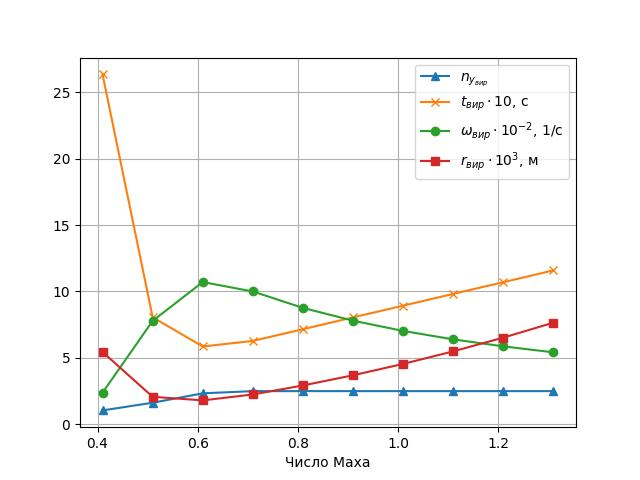
\includegraphics[width=6cm, height = 7cm]{../Оглавление/Part1/figures/РезультатыМаневры.jpg}}
    \end{minipage}  
    \begin{minipage}[c]{0.45\textwidth}
        \center{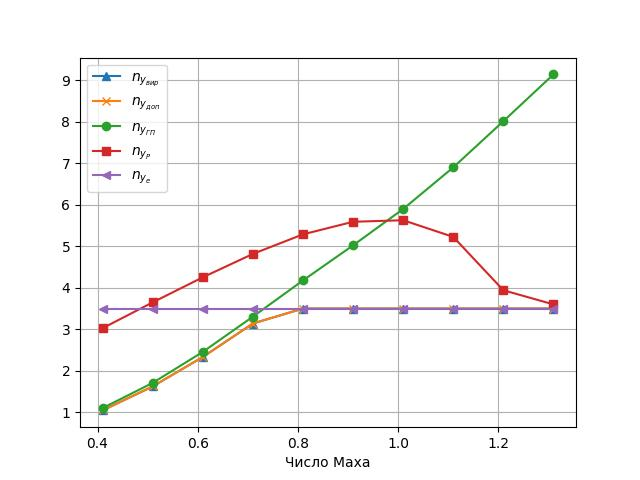
\includegraphics[width=6cm, height = 7cm]{../Оглавление/Part1/figures/РезультатыМаневры2.jpg}}
    \end{minipage}
\end{frame}